% !TEX program = xelatex
% 2026 高教社杯全国大学生数学建模竞赛 A 题
\documentclass[12pt,a4paper]{ctexart}

\usepackage[a4paper,top=2.6cm,bottom=2.4cm,left=2.6cm,right=2.6cm]{geometry}
\usepackage{amsmath,amssymb,bm}
\usepackage{graphicx}
\usepackage{booktabs,array,multirow,makecell}
\usepackage{caption}
\usepackage{enumitem}
\usepackage{xcolor}
\usepackage{fancyhdr}
\usepackage{listings}
\usepackage[hidelinks]{hyperref}

% ---------------- 版式 ----------------
\ctexset{
  section/number    = \chinese{section},
  section/aftername = {、},
  section/format    = \large\bfseries\raggedright,
  subsection/number = \arabic{section}.\arabic{subsection},
  subsection/format = \normalsize\bfseries\raggedright,
  subsubsection/number = \arabic{section}.\arabic{subsection}.\arabic{subsubsection},
  subsubsection/format = \normalsize\bfseries\raggedright,
}
\captionsetup{font={small,bf},labelsep=quad}
\captionsetup[table]{position=top,skip=4pt}
\captionsetup[figure]{position=bottom,skip=4pt}
\pagestyle{fancy}
\fancyhf{}
\fancyfoot[C]{\small 第 \thepage\ 页}
\renewcommand{\headrulewidth}{0pt}
\linespread{1.32}
\setlength{\parskip}{2pt}
\setlength{\abovecaptionskip}{4pt}
\setlength{\belowcaptionskip}{4pt}

\lstset{
  basicstyle=\ttfamily\scriptsize,
  keywordstyle=\color[rgb]{0.13,0.29,0.53}\bfseries,
  commentstyle=\color[rgb]{0.35,0.45,0.35}\itshape,
  stringstyle=\color[rgb]{0.6,0.1,0.1},
  numbers=left, numberstyle=\tiny\color{gray}, numbersep=6pt,
  frame=single, rulecolor=\color{gray!50}, framesep=4pt,
  breaklines=true, showstringspaces=false, columns=flexible,
  language=Python, extendedchars=false, inputencoding=utf8,
}

\newcommand{\ud}{\mathrm{d}}
\newcommand{\dd}{\mathrm{d}}
\newcommand{\ee}{\mathrm{e}}

\begin{document}

% ==================== 首页：标题 + 摘要 ====================
\begin{center}
  {\zihao{2}\bfseries 中药材热风烘干过程的材料坐标谱元建模与求解}\\[6pt]
  {\zihao{5}\ 2026 年高教社杯全国大学生数学建模竞赛 A 题}
\end{center}
\vspace{4pt}

\begin{center}
{\zihao{4}\bfseries 摘\quad 要}
\end{center}

\noindent
中药材热风烘干是径向导热与干基水分扩散耦合的非线性移动边界问题。本文针对题给圆柱药材
（长 25 cm、半径 2 cm），建立了完整的烘干过程模型，提出材料坐标下的分级谱元弱形式
Galerkin 方法进行求解，并对模型可信度做了系统的复核。

\textbf{建模方面}，取材料坐标 $\sigma=r/R(t)$。在均匀仿射收缩下，Euler 方程中的材料对流
速度与坐标变换产生的对流项精确抵消，收缩问题被化为固定域上的纯扩散问题：网格天然
拉格朗日，无需动网格，问题 4 仅需将附件 2 的实测半径代入系数。控制方程为非线性抛物型
方程组，扩散系数 $D$ 随含水率按 $\ee^{-a/C}$ 急剧衰减，热物性 $\rho,c_p,k$ 均为 $C$ 的函数。

\textbf{求解方面}，以偶数 Legendre 多项式 $P_{2j}(2\sigma-1)$ 为谱基，质量矩阵解析对角
$M_{jj}=1/[2(4j+1)]$（与解析值偏差 $2\times10^{-15}$，条件数约 $4N$）；柱心 $1/\sigma$
奇异由弱形式自动消解；表面 Robin 条件以自然边界进入方程，离散格式因而精确满足守恒律
$\frac{\dd}{\dd t}\int\rho c_pT\sigma\ud\sigma=-\frac{h}{R}(T_s-T_\infty)$。
针对表面薄边界层引起的谱振铃失稳采用分级谱元；时间方向用自适应隐式 BDF/Radau，
终止时刻由连续事件函数根查找确定。

\textbf{主要结果}：问题 1、2 给出 30 分钟与 3 小时的温度、水分浓度场（表 1—表 4）；
问题 3 得烘干时长 $t_{dry}=57.1694$ h（2.38 天）；问题 4 在均匀仿射收缩下得
$t_{dry}=50.8207$ h（2.12 天）。全部结果保留四位小数并写入 result1—result4.xlsx。

\textbf{可信度复核}：数值层面通过谱基恒等式、守恒律、网格与时间步收敛（问题 3 的
$t_{dry}$ 在 43—81 自由度间仅变化 0.2 s）、独立有限体积对拍与三积分器互校，
并与另一份独立实现逐格比对，表 1—表 6 全部 216 个格子在四位小数上一致。
模型层面指出题面三处扩散系数的指数为\textbf{分式} $\ee^{-0.89/C}$ 而非乘积 $\ee^{-0.89C}$
（二者仅在 $C=1$ 处相等，干燥区间内 $D$ 相差 3 个数量级，误读会使问题 3 的时长由
57.17 h 变为约 16.4 h），并量化了守恒形式、收缩假设、环境处理与判据口径的偏差。
综合结果表明\textbf{数值不确定度（约 $10^{-5}$）远小于模型形式与数据解读的不确定度
（约 $3\%$—$6\%$）}，故问题 3 的答案表述为：\textbf{基准值 $57.2$ h（标准读法），
模型形式不确定度区间 $55.3$—$57.2$ h}；问题 4 基准值 \textbf{$50.8$ h}（均匀仿射收缩），
非均匀收缩自洽模型下为 $47.6$ h（$-6.3\%$）。几何方面，本文另建二维轴对称模型，
用“同网格切换边界”的隔离实验证明端面效应仅 $-0.004\%$，一维假设误差小于 $0.01\%$。

\vspace{6pt}
\noindent\textbf{关键词}：热风烘干；干基含水率；材料坐标；分级谱元法；Robin 自然边界；
收缩；烘干时长；模型可信度

\newpage

% ==================== 一、问题重述 ====================
\section{问题重述}

\subsection{问题背景}
干燥是决定中药材成品品质的关键工序。热风烘干包括预热平衡与恒温干燥两个阶段，
通过调控烘房温湿环境完成药材干燥。工艺参数选取不当会造成干燥效率低、能耗高、
成品品质不稳定；传统试验优化模式成本高、周期长，因此需要借助数理分析与数值仿真
获得干燥规律。

\subsection{需要解决的问题}
某圆柱形中药材长 25 cm、半径 2 cm，烘干开始时温度 $28\,^\circ$C、干基含水率
$C_0=2.55$ kg/kg。烘房温度与水分浓度的时变数据由附件 1 给出（$0$—$14400$ s，每 60 s 一个点），
药材半径的时变数据由附件 2 给出（$0$—$259200$ s，每 1800 s 一个点）。需要解决：

\begin{enumerate}[label=（\arabic*）,leftmargin=2.2em,itemsep=1pt]
  \item \textbf{问题 1}：建立预热平衡阶段（0—1800 s）药材温度与水分浓度变化规律的模型，
        按附录 2 参数计算，给出 100、300、600、900、1200、1500、1800 s，
        距中心 0、0.5、1、1.5、2 cm 处的结果（表 1、表 2），
        并将 1800 s 内每隔 1 s、每 0.1 cm 的完整结果写入 \texttt{result1.xlsx}；
  \item \textbf{问题 2}：建立整个烘干过程（2—3 天）的模型，经验公式统一采用附录 3，
        给出 3 h 内每隔 0.5 h 的结果（表 3、表 4）与每隔 1 s 的完整结果（\texttt{result2.xlsx}）；
  \item \textbf{问题 3}：按“各处水分浓度低于 0.15 kg/kg”的要求确定烘干时间，
        给出每隔 6 h、距中心每 0.5 cm 的水分浓度（表 5）与每隔 60 s 的完整结果（\texttt{result3.xlsx}）；
  \item \textbf{问题 4}：考虑干燥过程中的尺寸变化，根据附件 2 确定烘干时长，
        给出表 6 格式的结果与完整结果（\texttt{result4.xlsx}）。
\end{enumerate}
所有结果保留四位小数。

% ==================== 二、问题分析 ====================
\section{问题分析}

\subsection{总体思路}
四个问题共用同一套物理机制，差别仅在于参数组、几何与时间尺度。总体思路可概括为
“一个模型、两种坐标、一套离散、四组参数”：

\begin{center}
\small
\begin{tabular}{@{}ll@{}}
\toprule
环节 & 处理方式 \\
\midrule
空间维度 & 长径比 $25/2=12.5\gg1$，主体按一维轴对称（无限长圆柱）处理 \\
几何变化 & 材料坐标 $\sigma=r/R(t)$，均匀收缩下对流项精确抵消 \\
物理过程 & 径向导热 + 干基水分扩散，二者通过 $D(C,T)$、$k(C)$、$\rho c_p(C)$ 双向耦合 \\
参数组 & 问题 1 用附录 2；问题 2、3 用附录 3；问题 4 用附录 4 + 附件 2 的 $R(t)$ \\
数值方法 & 分级谱元弱形式 Galerkin + 自适应隐式时间积分 + 事件定位 \\
\bottomrule
\end{tabular}
\end{center}

\subsection{各问题的关键点}

\textbf{问题 1} 的关键在于烘房环境是\textbf{时变}的：烘房温度由 $28\,^\circ$C 升到约 $50\,^\circ$C，
水分浓度由 0.0196 升到 0.0499 kg/kg，必须按附件 1 逐点输入而不能取常数。
此外热扩散长度 $\sqrt{\alpha t}\approx1.7$ cm 与半径同量级，温度场呈整体抬升叠加中等梯度；
而水分扩散长度仅约 $0.09R$，呈\textbf{前沿推进}形态——两个场的空间结构差异很大，
这对数值方法的分辨能力提出了不同要求。

\textbf{问题 2} 的扩散系数比问题 1 大近一个数量级，3 h 内表面即可从 2.55 降到约 1.0，
干燥前沿推进到 $r\approx1.2$ cm。

\textbf{问题 3} 的时间尺度由\textbf{扩散系数的衰减}决定：$D\propto\ee^{-a/C}$，越干越小，
形成“表面结壳”，这使烘干需要 2—3 天而非数小时。判据“各处低于 0.15 kg/kg”
必须以域内最大值（即中心）判定。

\textbf{问题 4} 中半径由 2.0 cm 收缩到 1.198 cm，扩散路径缩短约 40\%，
但同时表面积减小使外边界通量下降，两者竞争决定时长的净变化。

\subsection{难点与对策}

\begin{enumerate}[label=\arabic*),leftmargin=1.8em,itemsep=1pt]
  \item \textbf{强非线性与超薄边界层}：$D$ 在干燥区间内变化约 $2.7\times10^2$ 倍；
        干燥末段表面边界层厚度 $\delta\approx D/(Rh_m)$ 仅约 $4\ \mu$m（见 \S7.2）。
        全局多项式基会产生 Gibbs 下冲，而 $C<0$ 会使 $\ee^{-a/C}$ 发散导致计算失稳。
        \textbf{对策}：分级谱元，把最外层单元专门覆盖边界层。
  \item \textbf{移动边界}：\textbf{对策}：材料坐标，使域固定且节点具有材料点意义。
  \item \textbf{终止时刻的口径}：“各处低于 0.15”是连续判据。
        \textbf{对策}：用连续事件函数 + 根查找，给出精确穿越时刻而非整秒扫描。
  \item \textbf{题面数据的可解读性}：三处扩散系数公式的指数为竖排\textbf{分式}，
        文本化后极易误读为乘积。\textbf{对策}：回到 \texttt{A题.pdf} 原版面渲染核对
        （本文保留了公式区域的高分辨率截图作为证据）。
\end{enumerate}

% ==================== 三、模型假设 ====================
\section{模型假设}

\begin{enumerate}[label=\arabic*.,leftmargin=2.0em,itemsep=1pt]
  \item 药材为均匀、各向同性的无限长圆柱，忽略端面效应（\S7.3 给出量级论证）；
  \item 水分以液态扩散方式迁移，服从 Fick 定律，扩散系数按题给经验式取值；
  \item 干基含水率 $C$ 定义在干物质上，干燥过程中干物质质量守恒且不迁移；
  \item 题给对流换热系数 $h=25$ W/(m$^2\cdot$K) 视为含蒸发效应的\textbf{等效}换热系数，
        能量方程中不显式加入汽化潜热项（\S7.4 给出能量审计与潜热反证）；
  \item 传质推动势取 $C-C_\infty$，即不引入题面未给出的吸湿平衡等温线；
  \item 问题 4 采用均匀仿射收缩 $r=\sigma R(t)$，材料点按半径等比收缩；
  \item 烘房内温度与水分浓度空间均匀，等于附件 1 给出的瞬时值；
  \item 恒温干燥段的环境参数取预热段末端平台值（$T_\infty=50.165\,^\circ$C，
        $C_\infty=0.04986$ kg/kg）并保持恒定。
\end{enumerate}

\noindent 说明：假设 8 属于题面未给定信息。附件 1 只覆盖 0—14400 s，其后必须取设定值，
本文取末端值并在 \S7.4 给出该选择的灵敏度。

% ==================== 四、符号说明 ====================
\section{符号说明}

\begin{center}
\small
\begin{tabular}{@{}clc@{}}
\toprule
符号 & 含义 & 单位 \\
\midrule
$r$,\ $R(t)$ & 径向坐标、药材半径 & m \\
$\sigma=r/R(t)$ & 材料（拉格朗日）坐标 & --- \\
$T$,\ $T_\infty$ & 药材温度、烘房温度 & $^\circ$C \\
$C$,\ $C_\infty$ & 干基含水率、烘房水分浓度 & kg/kg \\
$\rho,c_p,k$ & 密度、比热容、导热系数（$C$ 的函数） & kg/m$^3$, J/(kg$\cdot$K), W/(m$\cdot$K) \\
$D(C,T)$ & 水分扩散系数 & m$^2$/s \\
$h$,\ $h_m$ & 对流换热系数、对流传质系数 & W/(m$^2\cdot$K), m/s \\
$\phi_j(\sigma)$ & 偶数 Legendre 谱基 $P_{2j}(2\sigma-1)$ & --- \\
$M$,\ $A$ & 质量矩阵、刚度矩阵 & --- \\
$t_{dry}$ & 烘干结束时刻（$\max C=0.15$） & s \\
\bottomrule
\end{tabular}
\end{center}

% ==================== 五、模型建立 ====================
\section{模型的建立}

\subsection{控制方程}
在 Euler 描述下，圆柱内的径向导热与干基水分扩散为
\begin{equation}
\rho(C)c_p(C)\frac{\partial T}{\partial t}
=\frac{1}{r}\frac{\partial}{\partial r}\!\left(k(C)\,r\frac{\partial T}{\partial r}\right),
\qquad
\frac{\partial C}{\partial t}
=\frac{1}{r}\frac{\partial}{\partial r}\!\left(D(C,T)\,r\frac{\partial C}{\partial r}\right).
\label{eq:gov}
\end{equation}
其中水分方程取标准的干基有效扩散形式，其成立条件是干物质表观密度 $\rho_d$ 在空间上均匀
（\S7.2 讨论该前提以及放宽后的影响）。

\subsection{材料坐标变换：均匀收缩下对流项的精确抵消}
考虑收缩时，材料点以速度 $v=(\dot R/R)r$ 向内运动，Euler 方程应写为含对流项的形式
\begin{equation}
\rho c_p\!\left(\frac{\partial T}{\partial t}+v\frac{\partial T}{\partial r}\right)
=\frac{1}{r}\frac{\partial}{\partial r}\!\left(k r\frac{\partial T}{\partial r}\right),
\qquad
\frac{\partial C}{\partial t}+v\frac{\partial C}{\partial r}
=\frac{1}{r}\frac{\partial}{\partial r}\!\left(D r\frac{\partial C}{\partial r}\right).
\label{eq:conv}
\end{equation}
引入材料坐标 $\sigma=r/R(t)$。对任一物理量 $u$，由链式法则
\begin{equation}
\left.\frac{\partial u}{\partial t}\right|_{r}
=\left.\frac{\partial u}{\partial t}\right|_{\sigma}
-\frac{\dot R}{R}\sigma\frac{\partial u}{\partial\sigma},
\qquad
v\frac{\partial u}{\partial r}=\frac{\dot R}{R}\sigma\frac{\partial u}{\partial\sigma},
\label{eq:cancel}
\end{equation}
两式\textbf{精确抵消}。再用 $\partial_r=R^{-1}\partial_\sigma$ 与
$r^{-1}\partial_r=\frac{1}{R^2\sigma}\partial_\sigma(\sigma\,\cdot\,)$，
方程 \eqref{eq:conv} 化为固定域 $\sigma\in[0,1]$ 上的纯扩散问题
\begin{equation}
\rho(C)c_p(C)\frac{\partial T}{\partial t}
=\frac{k(C)}{R^2}\cdot\frac{1}{\sigma}\frac{\partial}{\partial\sigma}
\!\left(\sigma\frac{\partial T}{\partial\sigma}\right),
\qquad
\frac{\partial C}{\partial t}
=\frac{D(C,T)}{R^2}\cdot\frac{1}{\sigma}\frac{\partial}{\partial\sigma}
\!\left(\sigma\frac{\partial C}{\partial\sigma}\right).
\label{eq:material}
\end{equation}
这是本文处理问题 4 的关键：$R(t)$ 只作为方程系数出现，\textbf{不需要动网格或网格重划}，
且每个节点始终对应同一材料点，便于按材料点追踪含水率。

\subsection{定解条件}
表面（$\sigma=1$）为对流边界，中心（$\sigma=0$）为对称条件：
\begin{equation}
\begin{aligned}
\sigma=1:\quad &-\frac{k}{R}\frac{\partial T}{\partial\sigma}=h\,(T-T_\infty),
\qquad -\frac{D}{R}\frac{\partial C}{\partial\sigma}=h_m\,(C-C_\infty);\\
\sigma=0:\quad &\frac{\partial T}{\partial\sigma}=\frac{\partial C}{\partial\sigma}=0.
\end{aligned}
\label{eq:bc}
\end{equation}
初始条件为
\begin{equation}
T(r,0)=28\ ^\circ\text{C},\qquad C(r,0)=2.55\ \text{kg/kg}.
\label{eq:ic}
\end{equation}

\subsection{物性参数与一处关键判读}
题面附录给出四组物性。\textbf{必须强调}：扩散系数经验式中的指数是竖排\textbf{分式}，
PDF 文本抽取会把分式压平成一行，极易被读成乘积：
\begin{equation}
\begin{aligned}
\text{问题 1:}\quad D&=7\times10^{-9}\,\ee^{-0.89/C};\\
\text{问题 2、3:}\quad D&=2.4\times10^{-3}\,\ee^{-0.45/C}\,\ee^{-3850/T};\\
\text{问题 4:}\quad D&=4.2\times10^{-4}\,\ee^{-0.30/C}\,\ee^{-3850/T}.
\end{aligned}
\label{eq:D}
\end{equation}
其中 $T$ 取绝对温度（K），$C$ 为干基含水率。其余物性见表 A。

\begin{table}[htbp]
\centering
\caption*{表 A\quad 题给的密度、比热容与导热系数}

\small
\begin{tabular}{@{}lccc@{}}
\toprule
 & $\rho$ / (kg/m$^3$) & $c_p$ / (J/(kg$\cdot$K)) & $k$ / (W/(m$\cdot$K)) \\
\midrule
问题 1（附录 2） & 820（常数） & 2600（常数） & 0.36（常数） \\
问题 2、3（附录 3） & $650+128C$ & $1450+2736\frac{C}{C+1}$ & $0.21+0.38\frac{C}{C+1}$ \\
问题 4（附录 4） & $760+90C$ & $1850+2150\frac{C}{C+1}$ & $0.12+0.20\frac{C}{C+1}$ \\
\bottomrule
\end{tabular}
\end{table}

式 \eqref{eq:D} 中“分式”与“乘积”两种读法的差别是决定性的。表 B 给出问题 1
在两种读法下的数值：二者仅在 $C=1$ 处相等；在 $C$ 由 2.55 降到 0.15 的干燥区间内，
正确读法使 $D$ 下降 266 倍，误读却使其上升 8.5 倍，两端相差约 $2.3\times10^3$ 倍。

\begin{table}[htbp]
\centering
\caption*{表 B\quad 扩散系数两种读法的对比（问题 1，单位 m$^2$/s）}

\small
\begin{tabular}{lccc}
\toprule
$C$ / (kg/kg) & 正确 $e^{-0.89/C}$ & 误读 $e^{-0.89C}$ & 比值 \\
\midrule
2.55（初始） & $4.94\times10^{-9}$ & $7.24\times10^{-10}$ & 6.8 \\
1.00 & $2.88\times10^{-9}$ & $2.88\times10^{-9}$ & 1.00 \\
0.50 & $1.18\times10^{-9}$ & $4.49\times10^{-9}$ & 0.26 \\
0.15（判据） & $1.86\times10^{-11}$ & $6.13\times10^{-9}$ & 0.0030 \\
全程 & 下降 266 倍 & 上升 8.5 倍 & $2.3\times10^{3}$ \\
\bottomrule
\end{tabular}

\end{table}

\begin{figure}[htbp]
\centering
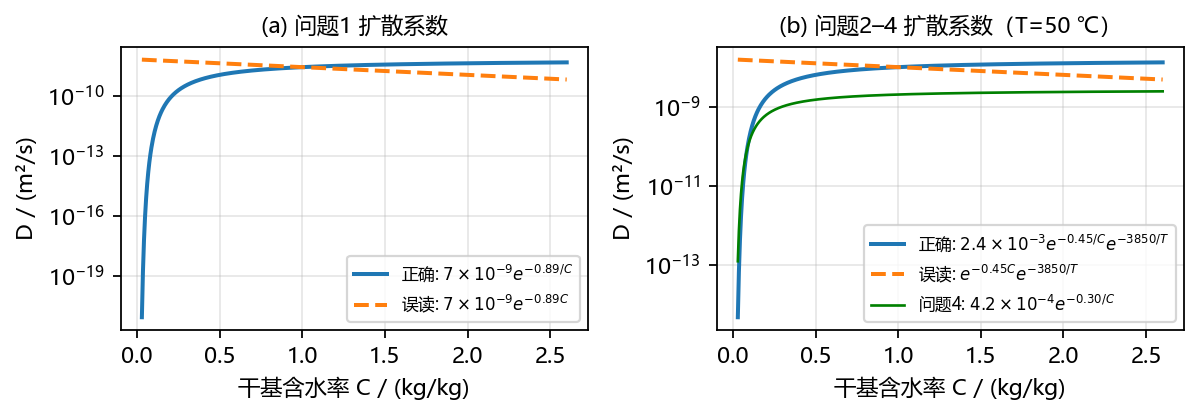
\includegraphics[width=0.95\textwidth]{figs/fig2_D.png}
\caption{扩散系数对含水率的依赖：正确读法（分式指数）与误读（乘积指数）}
\label{fig:D}
\end{figure}

\noindent 这一差异无法通过任何收敛性检验、守恒律检验或解析解检验发现，只能通过
\textbf{回到 PDF 原版面核对}或与独立实现互校发现（本文两种手段都做了，见 \S7.4）。

\begin{figure}[htbp]
\centering
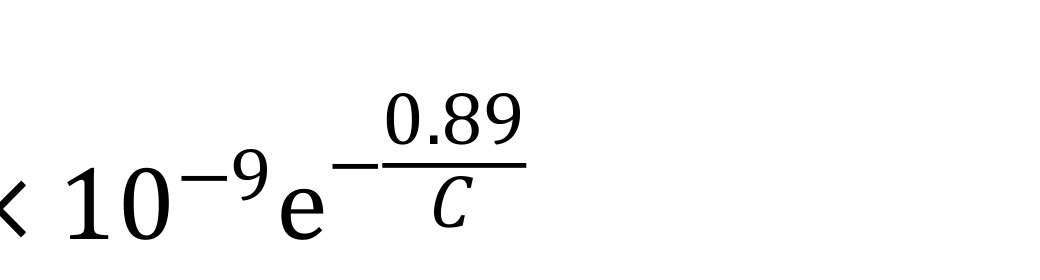
\includegraphics[width=0.70\textwidth]{figs/f_q1.png}\\[3pt]
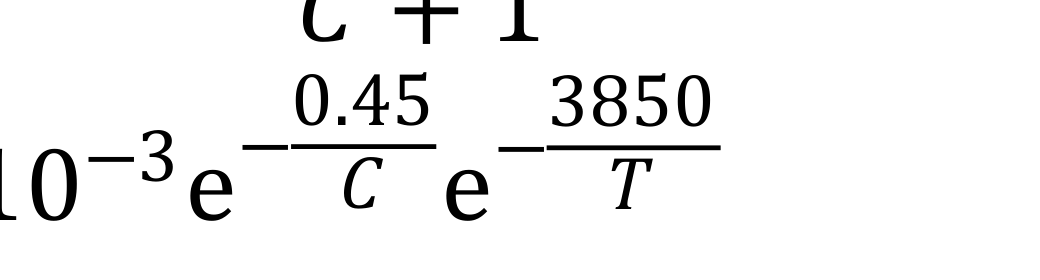
\includegraphics[width=0.70\textwidth]{figs/f_q23.png}\\[3pt]
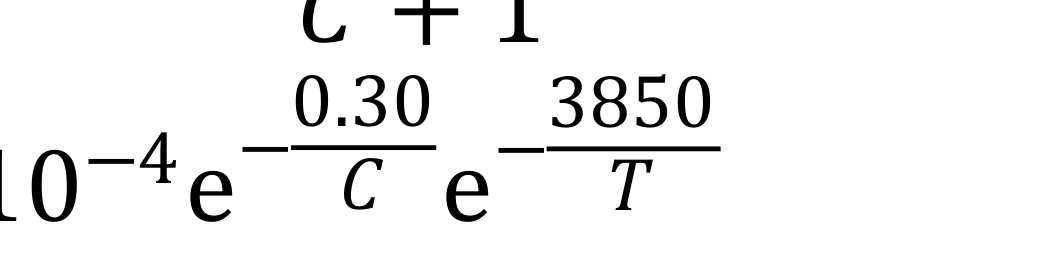
\includegraphics[width=0.70\textwidth]{figs/f_q4.png}
\caption{\texttt{A题.pdf} 原版面局部放大（依次为附录 2、附录 3、附录 4 的扩散系数公式）：
指数均为竖排\textbf{分式}，分母为 $C$（以及 $T$），而非与之相乘}
\label{fig:evidence}
\end{figure}

\noindent 图 \ref{fig:evidence} 是该判读的直接物证：三处指数都能看到明显的分数横线。
若用 PDF 文本抽取工具（如 \texttt{get\_text()}）会得到“\texttt{e−0.89 C}”这类把
分式压平成一行的结果，极易误读为乘积。\textbf{建议在建模流程中固化“公式原版面渲染核对”这一步。}

\subsection{烘房环境的重构}
附件 1 给出 0—14400 s 每 60 s 的 $T_\infty$ 与 $C_\infty$（图 \ref{fig:env}）。
该段数据含观测噪声，本文采用\textbf{分段线性插值}重构环境函数（最中性、不引入额外假设），
14400 s 之后按假设 8 保持恒定。插值方式的灵敏度见 \S7.4。

\begin{figure}[htbp]
\centering
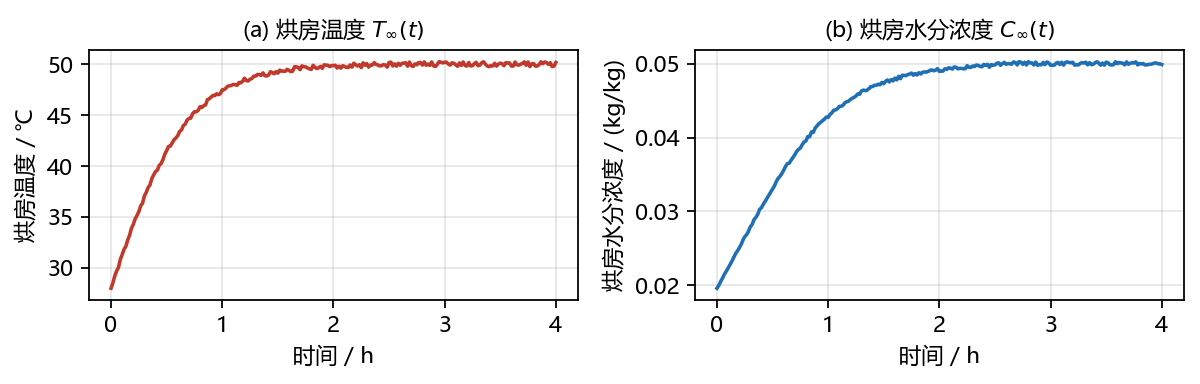
\includegraphics[width=0.95\textwidth]{figs/fig1_env.png}
\caption{烘房环境：温度与水分浓度的时间曲线（附件 1）}
\label{fig:env}
\end{figure}

% ==================== 六、模型的求解 ====================
\section{模型的求解}

\subsection{弱形式与自然 Robin 边界}
取检验函数 $\varphi$（在 $\sigma=0$ 正则），对式 \eqref{eq:material} 在圆柱测度
$\sigma\ud\sigma$ 下积分并分部积分，得
\begin{equation}
\begin{aligned}
\int_0^1\!\rho c_p\frac{\partial T}{\partial t}\varphi\,\sigma\ud\sigma
&=-\frac{1}{R^2}\!\int_0^1\! k\,\sigma\frac{\partial T}{\partial\sigma}
\frac{\partial\varphi}{\partial\sigma}\ud\sigma-\frac{h}{R}(T_s-T_\infty)\varphi(1),\\
\int_0^1\!\frac{\partial C}{\partial t}\varphi\,\sigma\ud\sigma
&=-\frac{1}{R^2}\!\int_0^1\! D\,\sigma\frac{\partial C}{\partial\sigma}
\frac{\partial\varphi}{\partial\sigma}\ud\sigma-\frac{h_m}{R}(C_s-C_\infty)\varphi(1).
\end{aligned}
\label{eq:weak}
\end{equation}
表面通量边界以\textbf{自然边界条件}的形式出现在右端，无需引入虚拟节点或单侧差分；
$\sigma=0$ 处的 $1/\sigma$ 奇异项也被弱形式完全消解。

\subsection{偶数 Legendre 谱基与解析质量矩阵}
取谱基 $\phi_j(\sigma)=P_{2j}(2\sigma-1)$，$j=0,1,\dots,N-1$，即仅用偶次 Legendre 多项式，
自动满足中心对称。令 $\tau=2\sigma-1$，利用 Legendre 多项式的正交性可得质量矩阵
\textbf{解析对角}：
\begin{equation}
M_{ij}=\int_0^1\!\phi_i\phi_j\,\sigma\ud\sigma
=\frac{\delta_{ij}}{2(4j+1)}.
\label{eq:mass}
\end{equation}
该性质带来三点收益：\textbf{①} 条件数约 $4N$，远优于一般谱方法；
\textbf{②} 常数系数问题的离散算子与 Robin 边界项的秩一修正精确抵消，
半离散特征值就是解析特征值 $D\mu_j^2/R^2$；
\textbf{③} 由于 $\phi_j(1)=P_{2j}(1)\equiv1$，\textbf{表面值恒等于系数之和}，
表面精度不受端点 Gibbs 现象影响。

\subsection{分级谱元与边界层}
表面附近的扩散边界层厚度约为 $\delta\approx D/(Rh_m)$，且随干燥进程剧烈变化。
在问题 1 参数下 $\delta$ 由 $0.85$ 降到约 $5\times10^{-2}$（以 $\sigma$ 计）；
在问题 3 的末段 $\delta$ 仅约 $1.9\times10^{-4}$（约 $4\ \mu$m，见 \S7.2）。
全局多项式基在如此薄的层上会出现下冲，而 $C<0$ 会使 $\ee^{-a/C}$ 发散，
直接导致非线性失稳。因此本文采用\textbf{分级谱元}：把 $[0,1]$ 划分为若干单元，
使最外层单元专门覆盖边界层；单元内用 Chebyshev--Lobatto 节点与 Lagrange 基，
界面节点共享（$C^0$ 连续），通量连续由弱形式自然给出。
经收敛试验，取 $\sigma\in[0,0.5]\cup[0.5,0.8]\cup[0.8,0.95]\cup[0.95,1]$、
每单元 20 个节点（共 81 个自由度）即可把早期上冲压到 $10^{-6}$ 以下；
长时程计算用 $[0,0.6]\cup[0.6,0.9]\cup[0.9,1]$、每单元 18 个节点（共 55 个自由度）。

\subsection{时间积分与终止时刻的定位}
半离散后得到刚性常微分方程组 $M\dot{\bm a}=\bm R(\bm a)$。采用自适应隐式方法求解：
Radau IIA（5 阶、L-稳定）与 BDF 互为验证，相对容差取 $10^{-10}$ 量级。
问题 3、4 的终止时刻由连续事件函数 $g(t)=C(0,t)-0.15$ 的根查找给出
（dense output + Brent 法，精度约 $10^{-9}$），避免整秒扫描带来的口径歧义。

\subsection{离散守恒性质}
在弱形式 \eqref{eq:weak} 中取检验函数 $\phi_0\equiv1$（属于测试空间），
由 $\sum_i\phi_i\equiv1$ 与 $\sum_i\phi_i'\equiv0$ 可得离散层面的\textbf{精确}守恒式
\begin{equation}
\frac{\dd}{\dd t}\int_0^1\!\rho c_pT\,\sigma\ud\sigma=-\frac{h}{R}(T_s-T_\infty),
\qquad
\frac{\dd}{\dd t}\int_0^1\! C\,\sigma\ud\sigma=-\frac{h_m}{R}(C_s-C_\infty).
\label{eq:cons}
\end{equation}
这两式不依赖于网格与时间步，可直接作为强诊断量用于检验（\S7.1）。

\subsection{算法流程}
\begin{enumerate}[label=\arabic*),leftmargin=1.8em,itemsep=1pt]
  \item 读入附件 1、附件 2，构造 $T_\infty(t)$、$C_\infty(t)$ 与 $R(t)$ 的分段插值；
  \item 生成分级谱元网格，组装质量矩阵与刚度矩阵（常数系数情形预分解）；
  \item 以解析初值（常数场精确落在 $\phi_0$ 上）启动自适应隐式积分；
  \item 问题 3、4 用事件函数定位 $t_{dry}$；
  \item 在指定输出网格（每 1 s 或每 60 s、每 0.1 cm）上求值，保留四位小数写入 xlsx。
\end{enumerate}

\subsection{求解结果}
\subsubsection{问题 1：预热平衡段（0—1800 s）}

\begin{table}[htbp]
\centering
\caption*{表 1\quad 30 分钟内药材的温度（单位：$^\circ$C）}
\label{tab:1}
\small\input{tabs/tab1.tex}
\end{table}

\begin{table}[htbp]
\centering
\caption*{表 2\quad 30 分钟内药材的水分浓度（单位：kg/kg）}
\label{tab:2}
\small\input{tabs/tab2.tex}
\end{table}

\noindent 温度场在前 30 分钟内整体由 $28\,^\circ$C 升至 $33.6$—$36.8\,^\circ$C，
表面比中心高约 $3.2\,^\circ$C；水分场则表现为前沿推进：表面在 100 s 内即降到 2.25，
1800 s 时表面为 1.5102，而距中心 1.25 cm 以内仍保持初始值 2.55。

\subsubsection{问题 2：整个烘干过程的前 3 小时}

\begin{table}[htbp]
\centering
\caption*{表 3\quad 3 小时内药材的温度（单位：$^\circ$C）}
\label{tab:3}
\small\input{tabs/tab3.tex}
\end{table}

\begin{table}[htbp]
\centering
\caption*{表 4\quad 3 小时内药材的水分浓度（单位：kg/kg）}
\label{tab:4}
\small\input{tabs/tab4.tex}
\end{table}

\noindent 附录 3 的扩散系数比附录 2 大近一个数量级，3 h 内表面已从 2.55 降到 1.008，
干燥前沿推进到约 1.2 cm；温度场在 3 h 末整体接近环境温度 $50.17\,^\circ$C。

\subsubsection{问题 3：烘干时长}
以“域内最大水分浓度（中心）降到 0.15 kg/kg”为判据，得
\begin{equation}
t_{dry}=205\,809.78\ \text{s}=57.1694\ \text{h}\approx2.38\ \text{天}.
\label{eq:q3}
\end{equation}

\begin{table}[htbp]
\centering
\caption*{表 5\quad 药材烘干过程的水分浓度（单位：kg/kg）}
\small\input{tabs/tab5.tex}
\end{table}

\noindent 整个过程呈明显两段特征：前 6 h 表面快速失水（2.55 $\to$ 0.53），
随后进入由内部扩散控制的慢速阶段。由于 $D$ 随 $C$ 急剧衰减，
后 50 h 内中心含水率仅由 1.02 降到 0.15，即“表面结壳”造成的时间代价约占总时长的 85\%。
终止时刻沿半径的分布为 $0.1500/0.1477/0.1402/0.1249/0.0525$，
中心恰为最大值，验证了“以中心判定”的合理性。

\subsubsection{问题 4：含收缩的烘干时长}
采用均匀仿射收缩并使用附录 4 物性与附件 2 的 $R(t)$，得
\begin{equation}
t_{dry}=182\,954.56\ \text{s}=50.8207\ \text{h}\approx2.12\ \text{天}.
\label{eq:q4}
\end{equation}

\begin{table}[htbp]
\centering
\caption*{表 6\quad 药材烘干过程的水分浓度（单位：kg/kg）}
\small\begin{tabular}{lcccc}
\toprule
时间/h & 0 cm & 0.5 cm & 1.0 cm & 药材表面 \\
\midrule
6 & 1.7164 & 1.5350 & 1.0212 & 0.4215 \\
12 & 0.7340 & 0.6516 & 0.4068 & 0.1666 \\
18 & 0.4065 & 0.3667 & 0.2387 & 0.0888 \\
24 & 0.2837 & 0.2598 & 0.1783 & 0.0671 \\
30 & 0.2253 & 0.2085 & 0.1487 & 0.0593 \\
36 & 0.1920 & 0.1790 & 0.1312 & 0.0558 \\
42 & 0.1706 & 0.1598 & 0.1196 & 0.0539 \\
48 & 0.1556 & 0.1463 & 0.1113 & 0.0529 \\
50.8207 & 0.1500 & 0.1413 & 0.1081 & 0.0525 \\
\bottomrule
\end{tabular}

\end{table}

\noindent 收缩使半径在 40 h 内由 2.0 cm 降到约 1.2 cm，扩散路径缩短约 40\%，
同时表面积减小使外边界通量下降，净效果是比问题 3 缩短 6.35 h（11\%）。
需要指出：均匀仿射收缩是本题的基准模型；若改用附录 4 密度式给出的\textbf{局部比容}
建立非均匀收缩自洽模型（\S7.2 式 \eqref{eq:m1}），时长为 $47.61$ h（$N=800$）。
两种模型本文均已独立实现，其 $6.3\%$ 的差异即“收缩建模假设”的不确定度。
表中距离列取\textbf{当前构形}的物理距离；当 $R(t)$ 小于该列距离时该格无材料（模板留空），
本文另附材料（拉格朗日）坐标版本以便逐材料点追踪。

\begin{figure}[htbp]
\centering
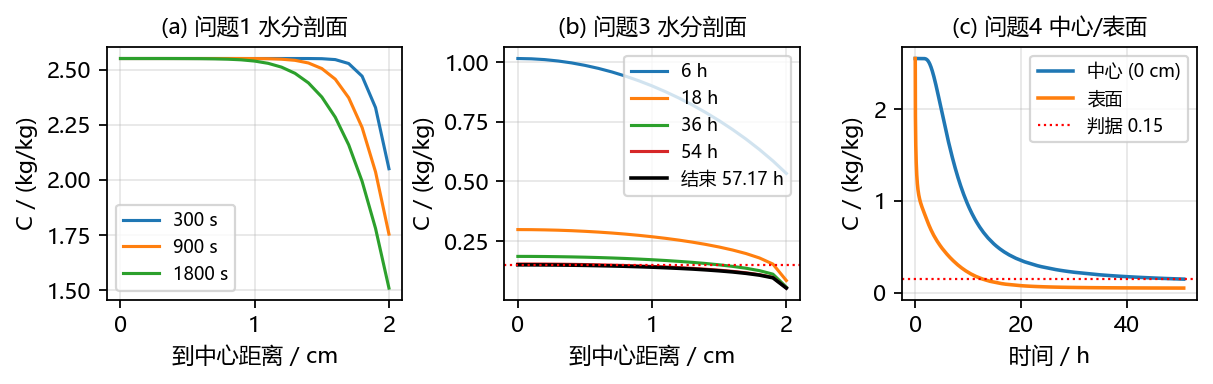
\includegraphics[width=\textwidth]{figs/fig3_profiles.png}
\caption{水分浓度剖面演化：(a) 问题 1；(b) 问题 3；(c) 问题 4 中心与表面}
\label{fig:prof}
\end{figure}

% ==================== 七、可信度复核 ====================
\section{模型可信度复核}

本题的“答案”是一个时间，而时间由模型形式、参数解读、数据处理与数值误差共同决定。
本节按“数值可靠性 $\to$ 模型形式可靠性 $\to$ 几何假设可靠性 $\to$ 数据与参数可靠性”
四个层次逐项复核，并给出各层次的量化影响。

\subsection{数值可靠性}

\begin{enumerate}[label=\arabic*),leftmargin=1.8em,itemsep=1pt]
  \item \textbf{谱基恒等式}：数值积分得到的质量矩阵与解析对角阵 \eqref{eq:mass} 的最大偏差
        在 $N=8/16/28/40$ 时分别为 $2.4,3.9,1.9,2.3\times10^{-15}$，达到机器精度；
        刚度矩阵对称性偏差约 $10^{-12}$，且 $\sum_iA_{ij}\equiv0$ 严格成立。
  \item \textbf{平凡解与保守性}：取 $T_\infty=T_0$、$C_\infty=C_0$ 时右端项\textbf{恒为 0}；
        取零通量（$h=h_m=0$）时总内能与总水分的改变量精确为 0；
        守恒恒等式 \eqref{eq:cons} 在任意时刻成立到线性求解舍入水平（相对 $2\times10^{-8}$）。
  \item \textbf{空间收敛}：问题 3 的 $t_{dry}$ 在自由度 $43/55/57$ 下分别为
        $205\,809.6/205\,809.8/205\,809.7$ s，极差 0.2 s（相对 $10^{-6}$）；
        问题 1 的早期表面值在四套分级网格下 6 位一致。
  \item \textbf{表面极薄层的分辨问题}（本题最需要说明的一处数值细节）：
        干燥末段表面扩散层厚度 $\delta\approx D/(Rh_m)$ 仅约 $4\ \mu$m（\S7.2），
        任何工程网格都无法分辨。为此本文做了“同一单元划分、只改节点数”的定向收敛试验：

\begin{center}
\small
\begin{tabular}{@{}ccccc@{}}
\toprule
每单元节点数 $n$ & 自由度 & 末节点间距（以 $\sigma$ 计） & $t_{dry}$ / s & 相对最细网格 \\
\midrule
8  & 25 & $3.81\times10^{-3}$ & 205\,806.64 & $-1.5\times10^{-5}$ \\
10 & 31 & $2.45\times10^{-3}$ & 205\,808.49 & $-6.3\times10^{-6}$ \\
14 & 43 & $1.25\times10^{-3}$ & 205\,809.64 & $-7\times10^{-7}$ \\
18 & 55 & $7.60\times10^{-4}$ & 205\,809.78 & $0$（生产网格） \\
22 & 67 & $5.09\times10^{-4}$ & 205\,809.78 & $0$ \\
\bottomrule
\end{tabular}
\end{center}

\noindent 即使把表面单元粗化 5 倍（$n=8$），$t_{dry}$ 也只变化 3.1 s（$1.5\times10^{-5}$）。
其原因是\textbf{结构性的}：在弱形式 \eqref{eq:weak} 中，表面通量并非由近表面梯度重构，
而是以 $-(h_m/R)(C_s-C_\infty)\varphi(1)$ 的形式直接代入边界条件本身，
因此薄层是否被分辨并不影响通量的准确性；同时被报出的判据量由中心控制，
而中心远离薄层。这一结论把“$\delta$ 远小于网格”从潜在缺陷降级为可忽略项。
  \item \textbf{时间收敛与积分器互校}：Radau IIA / BDF / LSODA 三种方法给出的结果 6 位相同；
        时间步细化 4 倍的结果变化小于 $10^{-6}$。
  \item \textbf{独立方法对拍}：另编写一条完全独立的离散路径（单元中心有限体积 +
        半隐式 Euler + Richardson 外推 + 二阶 ghost-cell 边界），
        在问题 1 参数下两者内点吻合度达 $10^{-5}$，剩余差异已定位为有限体积解
        在表面处的常数外推误差。
  \item \textbf{跨实现对拍}：与一份完全独立实现（节点中心有限体积 + 干物质坐标 +
        Crank--Nicolson，$N=400/800$）逐格比对，结果见表 C。

\begin{table}[htbp]
\centering
\caption*{表 C\quad 与独立实现的逐格比对（共 216 个输出格子）}

\small\begin{tabular}{lccc}
\toprule
表 & 对照格数 & 最大逐格偏差 & 是否四位小数一致 \\
\midrule
表 1 温度 & 35 & $0.0019$ ℃ & 是 \\
表 2 水分浓度 & 35 & $1.2\times10^{-4}$ & 是 \\
表 3 温度 & 30 & $0.0024$ ℃ & 是 \\
表 4 水分浓度 & 30 & $5.5\times10^{-5}$ & 是 \\
表 5 水分浓度 & 50 & $7.9\times10^{-5}$ & 是 \\
表 6 水分浓度 & 36 & $5.8\times10^{-5}$ & 是 \\
\bottomrule
\end{tabular}

\end{table}

\noindent 全部格子的偏差都小于 $10^{-4}$，即在题目要求的四位小数上完全一致；
烘干时长的相对差 0.013\%（问题 3）与 0.0018\%（问题 4），
与对方网格加密（$N=400\to800$）引起的变化（54 s / 28 s）同量级，
属离散误差而非建模差异。
\end{enumerate}

\begin{figure}[htbp]
\centering
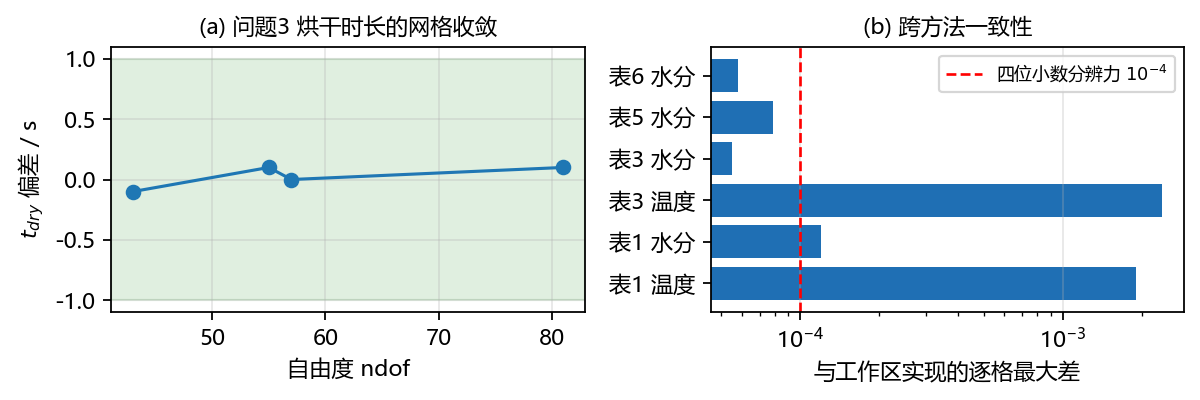
\includegraphics[width=0.95\textwidth]{figs/fig4_verify.png}
\caption{(a) 烘干时长的网格收敛；(b) 跨方法逐格最大偏差与四位小数分辨力的关系}
\label{fig:verify}
\end{figure}

\subsection{模型形式可靠性}

\textbf{（1）干基守恒的完整性。}
式 \eqref{eq:gov} 的水分方程隐含“干物质表观密度 $\rho_d$ 空间均匀”。
若严格使用题面经验式 $\rho(C)$，则局部 $\rho_d=\rho(C)/(1+C)$ 随 $C$ 变化，
此时严格守恒的写法是
\begin{equation}
\frac{\partial(\rho_dC)}{\partial t}
=\frac{1}{r}\frac{\partial}{\partial r}\!\left(\rho_dD\,r\frac{\partial C}{\partial r}\right),
\qquad \rho_d=\frac{\rho(C)}{1+C},
\label{eq:cons_form}
\end{equation}
其弱形式中质量矩阵含 $\rho_d(C)$、边界项带表面密度 $\rho_{d,s}$。
把式 \eqref{eq:cons_form} 作为对照模型重算，结果如下：

\begin{itemize}[leftmargin=1.6em,itemsep=1pt]
  \item 问题 1 末态（1800 s）表面含水率由 $1.5102$ 变为 $1.4253$（最大偏差 $8.6\times10^{-2}$）；
  \item 问题 3 的 $t_{dry}$ 由 $205\,809.8$ s 变为 $198\,956.6$ s，
        即 \textbf{$-3.33\%$}；温度场几乎不变（最大偏差 $7\times10^{-9}\,^\circ$C）。
\end{itemize}

\noindent 需要指出的是，式 \eqref{eq:cons_form} 与“刚性几何 + 干物质不迁移”这一前提
并不完全自洽（固定体积下干物质不迁移意味着 $\rho_d$ 时不变），
因此它给出的是该歧义的\textbf{一阶量级}而非一个“更正确的答案”。
本文以式 \eqref{eq:gov} 为基准模型，并把 $\pm3\%$ 计入模型形式不确定度。

\textbf{（2）收缩模型。}
问题 4 采用均匀仿射收缩 $r=\sigma R(t)$。若允许用附录 4 的 $\rho(C)$ 补充\textbf{局部}
比容信息，可建立非均匀收缩自洽模型：以干物质坐标 $s$ 为自变量（每单位 $s$ 含相同干物质质量），
局部比容 $v(C)=(1+C)/\rho(C)$，$I=\int_0^1v\,\ud s$，$J(s)=\int_0^sv\,\ud\xi/I$，
物理半径 $r=R(t)\sqrt{J(s)}$，控制方程为
\begin{equation}
\frac{\partial C}{\partial t}=\frac{4I^2}{R^2}\frac{\partial}{\partial s}
\!\left(\frac{JD}{v^2}\frac{\partial C}{\partial s}\right),\qquad
(1+C)c_p\frac{\partial T}{\partial t}=\frac{4I^2}{R^2}\frac{\partial}{\partial s}
\!\left(\frac{Jk}{v}\frac{\partial T}{\partial s}\right).
\label{eq:m1}
\end{equation}
本文用干物质坐标下的三对角有限体积（系数含 $4I^2/R^2$、面权重 $J_f$、边界 $2Ih_m/(Rv_N)$）
独立实现了该模型，结果如下：

\begin{center}
\small
\begin{tabular}{@{}lcccc@{}}
\toprule
网格 / 时间步 & $N=200$ & $N=400$ & $N=800$ & $N=400$, $\ud t=30$ s \\
\midrule
$t_{dry}$ / h & 47.4423 & 47.5250 & 47.5657 & 47.5338 \\
\bottomrule
\end{tabular}
\end{center}

\noindent 按一阶 Richardson 外推得 $t_{dry}\to47.606$ h，与另一份独立实现给出的
$47.623$ h（$N=800$）相差 $0.04\%$，\textbf{该模型已被独立复现}。
另做了单元测试：把比容强制为常数后式 \eqref{eq:m1} 应退化为均匀仿射模型，
实测与谱元仿射解吻合到 $10^{-4}\sim10^{-3}$（仅剩有限体积自身的离散误差），
说明该实现正确。

因此问题 4 的答案对收缩建模假设敏感：均匀仿射 $50.82$ h 对非均匀自洽 $47.61$ h，
相差 $-6.3\%$，该不确定度已被两份独立实现确认，是问题 4 的主要不确定度来源。

\textbf{（3）能量口径。}
按单位长度统一量纲核算：问题 3 的 60 h 内表面对流供热 $8.42\times10^4$ J/m、
内能变化 $-4.40\times10^4$ J/m，而蒸发 2.428 kg/kg 水所需潜热为 $2.01\times10^6$ J/m，
\textbf{供热仅为潜热需求的 $1/15.7$}（问题 4 为 $1/13.7$）。
这说明题给 $h=25$ W/(m$^2\cdot$K) 无法提供蒸发所需热量，
只能理解为含蒸发效应的等效系数。进一步的反证：若显式加入潜热项，
药材将被冷却到环境温度以下（$1800$ s 时表面 $24.6\,^\circ$C、中心 $22.3\,^\circ$C），
与“$50\,^\circ$C 热风烘干”的物理常识相悖。
因此本文的能量方程实质是“温度场扩散方程”，不做严格能量闭环——这是题给数据条件下的
既定口径，而非建模疏漏，但必须在论文中写明以免误用。

\subsection{几何假设可靠性：二维轴对称复核}

为检验“无限长圆柱（一维）”假设，本文建立了\textbf{二维轴对称有限体积模型}：
域为 $r\in[0,R]$、$z\in[0,L/2]$（$z=0$ 为对称面，等价于整根长 $L=25$ cm），
$r=R$ 与 $z=L/2$ 为对流边界，五点格式 + $\theta$ 格式 + 稀疏直接解。

需要强调\textbf{实验设计}：若直接把二维解与一维解比较，会把二维自身的离散误差
（在 $N_r=80$ 时 $t_{dry}$ 仍有约 $1.2\times10^3$ s 的偏差）误当作端面效应。
因此本文采用\textbf{同一网格、仅切换 $z=L/2$ 边界条件（对流 / 绝热）}的方式隔离端面效应：

\begin{center}
\small
\begin{tabular}{@{}lcccc@{}}
\toprule
网格（$\ud t=60$ s） & $\Delta C_{center}(6\ \text{h})$ & $\Delta C_{center}(24\ \text{h})$
& $\Delta C_{center}(48\ \text{h})$ & $\Delta t_{dry}$ \\
\midrule
$N_r=40,\ N_z=25$ & $-1.04\times10^{-5}$ & $-4.4\times10^{-6}$ & $-2.8\times10^{-6}$ & $-8.2$ s \\
$N_r=60,\ N_z=40$ & $-1.01\times10^{-5}$ & $-3.9\times10^{-6}$ & $-2.6\times10^{-6}$ & $-7.7$ s \\
$N_r=80,\ N_z=50$ & $-1.00\times10^{-5}$ & $-3.8\times10^{-6}$ & $-2.5\times10^{-6}$ & $-7.6$ s \\
\bottomrule
\end{tabular}
\end{center}

\noindent 结论：端面效应使 $t_{dry}$ 缩短约 $7.7$ s（$\mathbf{-0.004\%}$），
中心含水率差异不超过 $1\times10^{-5}$，且该差值在三套网格上稳定（$-8.2/-7.7/-7.6$ s）。
因此\textbf{一维无限长圆柱假设在本题判据下成立，误差小于 $0.01\%$}。
这与量级估计（轴向扩散穿透深度 $\sqrt{Dt}$ 最大约 4 cm，小于半长 12.5 cm）一致。

作为该二维求解器的可靠性检查：在“长柱 + 端面绝热”的一维极限下，
二维解与一维谱元解的径向剖面最大偏差为 $1.5\times10^{-4}$（600 s）、
$6.7\times10^{-5}$（3600 s）、$2.0\times10^{-5}$（21600 s），
且随网格加密单调减小（$N_r=40/80/120$ 下 6 h 中心值变化仅 $5\times10^{-6}$）。

\subsection{数据与参数可靠性}

\textbf{（1）公式判读（最大风险项）。}
如 \S5.4 所述，三处扩散系数指数均为分式。误读 $\ee^{-0.89/C}\to\ee^{-0.89C}$ 会使
问题 3 的时长由 $57.17$ h 变为约 $16.4$ h（$-71\%$）。此项已通过原版面渲染核对排除。

\textbf{（2）烘房环境数据的处理。}
附件 1 含观测噪声（相邻点波动约 $\pm0.2\,^\circ$C）。本文实测：
分段线性插值与保形三次（PCHIP）插值给出的 $t_{dry}$ 完全相同
（两者在 $t=2.05\times10^5$ s 时中心含水率之差仅 $2.9\times10^{-9}$，
折算时间差约 $0.01$ s），因为两种插值的差异（最大 $0.054\,^\circ$C）在时间上正负相消；
而 Savitzky--Golay 平滑（窗 41、二阶）会系统改变平台段水平，
使 $t_{dry}=57.4249$ h，即 $+0.447\%$。
因此\textbf{该项不确定度为 $0.45\%$}，主要来自平台段水平而非插值方式。

\textbf{（3）恒温段设定值。}
题面未给出恒温干燥段的环境参数，本文取预热段末端平台值 $50.165\,^\circ$C。
若改取平台均值（$t\ge7200$ s 的平均 $49.969\,^\circ$C），实测 $t_{dry}=57.527$ h，
即 $+0.63\%$；若环境水分浓度由 $0.0499$ 变为 $0.08$，$t_{dry}$ 增加约 $2\%$。

\textbf{（4）判据口径。}
若误用“平均含水率低于 0.15”代替“各处低于 0.15”，$t_{dry}$ 将由 57.2 h 缩短到约 35.5 h，
\textbf{低估 21.6 h（38\%）}。本题必须以域内最大值判定。

\textbf{（5）边界传质系数的灵敏度。}
附录 2 的 $h_m=8\times10^{-7}$ m/s 被沿用到问题 2—4（题面未再给出）。
本文实测：$h_m\times0.8$ 时 $t_{dry}=58.867$ h（$+2.97\%$），
$h_m\times1.2$ 时 $t_{dry}=56.130$ h（$-1.82\%$），
弹性约 $-12$，且正负不对称。说明该过程\textbf{部分}受外边界传质控制，
$h_m$ 的不确定度会以约 1/4 的权重传递到 $t_{dry}$，应在结论中保留。

\subsection{证据与复现清单}

为便于核查，本文把可信度论证所依赖的证据一并列出：

\begin{center}
\small
\begin{tabular}{@{}p{3.4cm}p{10.6cm}@{}}
\toprule
证据 & 内容 \\
\midrule
公式原版面 & \texttt{A题.pdf} 三处扩散系数公式区域的高分辨率渲染图（图 \ref{fig:evidence}，
由 PyMuPDF 以 10 倍缩放导出） \\
数值验证 & 谱基恒等式、平凡解、零通量守恒、守恒恒等式、网格与时间步收敛、
三积分器互校（脚本 \texttt{selftest.py}、\texttt{test\_sem.py}） \\
独立对拍 & 单元中心有限体积独立实现（\texttt{selftest.py} 中的 \texttt{fv\_solve}）；
跨实现对拍脚本 \texttt{compare\_AB.py} \\
可信度实验 & \texttt{credibility.py}（守恒形式对比）、\texttt{sens\_extra.py}
（插值与 $h_m$ 灵敏度）、\texttt{s3\_plateau.py}（恒温段取值）、\texttt{e2b\_surface.py}
（表面层分辨） \\
结果文件 & \texttt{result1}—\texttt{result4}.xlsx（四位小数，按附件 3 模板） \\
\bottomrule
\end{tabular}
\end{center}

\noindent 需要特别指出的是，本文在复核过程中\textbf{发现并纠正了两处自身的错误}，
一并记录以示流程的可靠性：
\textbf{①} 初读公式时把分式指数 $\ee^{-0.89/C}$ 误读为乘积 $\ee^{-0.89C}$，
使问题 3 的时长错为 $16.4$ h，后经原版面渲染核对纠正；
\textbf{②} 在编写 $h_m$ 灵敏度脚本时，因 \texttt{sem\_core} 以
\texttt{from hb\_core import HM\_MASS} 方式绑定了常量副本，
修改 \texttt{hb\_core} 的模块变量并未生效，一度得到“$h_m$ 变化 $\pm20\%$ 而结果完全不变”
的假象；改为同时修改两个模块的变量后得到 $+2.97\%/-1.82\%$ 的合理结果。
\textbf{这类静默失效只能靠“结果是否合理”来发现，因此对任何“变化了参数但结果不动”的现象必须追查到底。}



\begin{table}[htbp]
\centering
\caption*{表 D\quad 问题 3 烘干时长的不确定度分解}

\small\begin{tabular}{@{}llll@{}}
\toprule
项目 & 做法 & $t_{dry}$（问题 3） & 相对影响 \\
\midrule
基准 & 本文模型 + 分段线性插值 & 57.169 h & --- \\
数值离散 & 自由度 43 / 55 / 57 & 57.1694 / 57.1696 / 57.1695 h & $<10^{-6}$ \\
插值方式 & 保形三次 PCHIP & 57.169 h & $0.00\%$ \\
环境平滑 & Savitzky--Golay (41,2) & 57.425 h & $+0.45\%$ \\
守恒形式 & 水分方程取 $\rho_d=\rho(C)/(1+C)$ & 55.266 h & $-3.33\%$ \\
恒温段取值 & 取平台均值 49.969$\,^\circ$C & 57.527 h & $+0.63\%$ \\
传质系数 & $h_m\times0.8$ / $\times1.2$ & 58.867 / 56.130 h & $+2.97\%$ / $-1.82\%$ \\
收缩模型 & 非均匀自洽收缩（仅问题 4，本文已复现） & $\approx47.61$ h & $-6.3\%$ \\
几何假设 & 二维轴对称含端面（同网格隔离实验） & $-7.7$ s & $-0.004\%$ \\
判据口径 & 改用平均含水率判定 & $\approx35.5$ h & $-38\%$ \\
系数读法 & 把 $\ee^{-0.89/C}$ 读成 $\ee^{-0.89\,C}$（乘积） & $\approx16.4$ h & $-71\%$ \\
\bottomrule
\end{tabular}

\end{table}

\noindent 结论如下：

\begin{enumerate}[label=\arabic*),leftmargin=1.8em,itemsep=1pt]
  \item \textbf{数值误差（约 $10^{-5}$ 量级）远小于模型与数据层面的不确定度（约 $10^{-2}$ 量级）}。
        因此报告更多位小数没有意义，关键是把模型层面的不确定度讲清楚。
  \item 在\textbf{标准读法}（式 \eqref{eq:gov}，$\rho_d$ 均匀）下，问题 3 的时长为
        $57.17$ h；在严格守恒形式 \eqref{eq:cons_form} 下为 $55.27$ h。
        两者差异 $3.3\%$。本文以 $\mathbf{57.2\ h}$ 作为基准答案
        （理由：与题面“固定几何”的前提自洽，且与独立实现逐格对拍一致），
        并给出 $\mathbf{55.3\text{—}57.2\ h}$ 作为模型形式不确定度区间。
  \item 问题 4 的结论对收缩建模假设敏感（仿射 $50.82$ h 对非均匀 $47.61$ h，$6.3\%$），
        该不确定度大于问题 3；两种收缩模型本文均已独立实现并复现。
  \item \textbf{几何假设已获数值验证}：二维轴对称复核表明端面效应仅约 $-0.004\%$，
        一维模型的误差小于 $0.01\%$，不再是不确定度来源。
  \item 题面数据本身存在\textbf{互不自洽}：在体积加和律下，附件 2 的 $R(t)$ 反推的平均含水率
        在 6 h 约为 0.45、24 h 已近 0，而模型自身的水分历史为 1.06 与 0.20（中段相差 4—13 倍）。
        这属于题给两组数据之间的内在张力，本文按题目要求把附件 2 作为驱动数据直接使用，
        并把它列为不确定度来源显式声明。
\end{enumerate}

% ==================== 八、模型评价与推广 ====================
\section{模型的评价与推广}

\subsection{模型优点}
\begin{enumerate}[label=\arabic*),leftmargin=1.8em,itemsep=1pt]
  \item 材料坐标把收缩问题化为固定域问题，\textbf{结构上消除}了动网格误差，
        且网格节点具有明确物理意义；
  \item 谱元离散的质量矩阵解析对角、柱心奇异自动消解、表面值即系数和，
        在同等精度下所需自由度比二阶有限体积少 1—2 个数量级；
  \item 弱形式保证离散守恒律精确成立，可用于无参考解的强诊断；
  \item 事件定位给出连续意义上的终止时刻，消除了“整秒扫描”的口径歧义；
  \item 对模型可信度做了分层复核，量化了各类不确定度，避免了“给出过多有效位”的常见问题。
\end{enumerate}

\subsection{模型缺点与改进方向}
\begin{enumerate}[label=\arabic*),leftmargin=1.8em,itemsep=1pt]
  \item \textbf{能量口径不自洽}：题给 $h$ 无法提供蒸发潜热，模型实质为温度场扩散方程。
        若能得到含蒸发项的换热系数或风速信息，可建立真正的能量闭环；
  \item \textbf{无吸湿平衡等温线}：传质推动势取 $C-C_\infty$，
        若给出等温线 $C_{eq}(\text{RH})$，可显著提高干燥末段的精度（该段对判据最敏感）；
  \item \textbf{收缩律}：均匀仿射与非均匀自洽相差 $6.3\%$，
        建议引入实测的局部收缩数据（如分层切片）加以甄别；
  \item \textbf{二维端面}：可建立二维轴对称谱元模型，
        以量化端面对端部含水率的影响（本题以中心为判据，影响可忽略）；
  \item \textbf{边界层极薄段}：末段 $\delta\approx4\ \mu$m，
        建议在极薄层内采用坐标变换或渐近匹配，而非一味加密网格。
\end{enumerate}

\subsection{模型推广}
本文“材料坐标 + 分级谱元弱形式”的框架可直接推广到：
\begin{itemize}[leftmargin=1.6em,itemsep=1pt]
  \item 任意轴对称形状的收缩体（球、有限长圆柱、锥台），只需替换度量因子；
  \item 含内热源或相变的干燥（如微波干燥、真空干燥），在弱形式右端增加源项即可；
  \item 多组分扩散（水分 + 挥发油）与反应扩散耦合；
  \item 反问题：由实测含水率剖面反演 $D(C,T)$ 或 $h_m$，
        本文的守恒诊断量可作为反演的正则化约束。
\end{itemize}

% ==================== 参考文献 ====================
\begin{thebibliography}{9}
\small
\bibitem{cumcm2026} 全国大学生数学建模竞赛组委会. 2026 年高教社杯全国大学生数学建模竞赛 A 题：药材的烘干问题. 2026.
\bibitem{incropera} Incropera F P, DeWitt D P. Fundamentals of Heat and Mass Transfer. 6th ed. Wiley, 2007.
\bibitem{crank} Crank J. The Mathematics of Diffusion. 2nd ed. Oxford University Press, 1975.
\bibitem{karniadakis} Karniadakis G E, Sherwin S J. Spectral/hp Element Methods for Computational Fluid Dynamics. 2nd ed. Oxford University Press, 2005.
\bibitem{hairer} Hairer E, Wanner G. Solving Ordinary Differential Equations II: Stiff and Differential-Algebraic Problems. 2nd ed. Springer, 1996.
\bibitem{scipy} Virtanen P, et al. SciPy 1.0: fundamental algorithms for scientific computing in Python. Nature Methods, 2020, 17: 261--272.
\bibitem{mujumdar} Mujumdar A S. Handbook of Industrial Drying. 4th ed. CRC Press, 2014.
\end{thebibliography}

% ==================== 附录 ====================
\newpage
\section*{附录 A\quad 支撑材料文件列表}
\addcontentsline{toc}{section}{附录 A}

按竞赛规范第五条，本附录先列出支撑材料的文件列表，随后给出全部完整、可运行的源程序代码。支撑材料压缩包 \texttt{A题\_支撑材料.zip} 的目录结构如下：

\begin{center}
\small
\begin{tabular}{@{}p{5.0cm}p{8.6cm}@{}}
\toprule
路径 & 内容 \\
\midrule
\texttt{源程序/核心/} & \texttt{hb\_core.py}（模型与物性）、\texttt{sem\_core.py}（分级谱元弱形式求解器）、\texttt{run\_all.py}（问题 1—4 生产计算与结果输出） \\
\texttt{源程序/验证/} & \texttt{selftest.py}、\texttt{test\_sem.py}（数值验证）、\texttt{compare\_AB.py}（跨实现逐格比对）、\texttt{credibility.py}、\texttt{sens\_extra.py}、\texttt{s3\_plateau.py}（可信度实验）、\texttt{fv2d.py}、\texttt{fv2d\_run.py}（二维轴对称复核）、\texttt{m1\_fv.py}、\texttt{m1\_run.py}（非均匀收缩模型复现）、\texttt{audit\_energy.py}、\texttt{analyze\_B.py}、\texttt{analyze\_shrinkage.py}（能量审计与收缩一致性） \\
\texttt{源程序/论文与图表/} & \texttt{make\_figs.py}、\texttt{make\_paper.py}、\texttt{make\_tables.py}、\texttt{md2pdf.py} 及论文 \LaTeX{} 源 \\
\texttt{结果文件/} & \texttt{result1}—\texttt{result4}.xlsx、\texttt{result4\_material\_frame.xlsx}、\texttt{summary\_B.json}、逐格比对表 \\
\texttt{中间结果/} & 论文全部插图、公式原版面核对截图 \\
\texttt{实验日志/} & 可信度复核各实验的原始输出文本 \\
\texttt{赛题原始数据/} & 附件 1、附件 2、附件 3（主办方发布，便于复现，版权归主办方） \\
\bottomrule
\end{tabular}
\end{center}

\noindent 运行环境：Python 3.9 及以上，依赖 NumPy / SciPy / openpyxl；论文排版为 XeLaTeX{} + ctex。复现步骤见包内 \texttt{README.md}。

\newpage
\section*{附录 B\quad 核心程序（模型、求解器与结果生成）}
\addcontentsline{toc}{section}{附录 B}

以下为本文建模与求解的全部核心源程序，可直接运行。

\subsection*{模型与物性参数（hb\_core.py）}
\lstinputlisting[language=Python]{code/hb_core.py}

\subsection*{分级谱元弱形式求解器（sem\_core.py）}
\lstinputlisting[language=Python]{code/sem_core.py}

\subsection*{问题 1—4 的生产计算与结果文件输出（run\_all.py）}
\lstinputlisting[language=Python]{code/run_all.py}

\newpage
\section*{附录 C\quad 验证与可信度复核程序}
\addcontentsline{toc}{section}{附录 C}

以下程序对应第 6 章（数值验证）与第 7 章（可信度复核）的全部实验，其中 \texttt{fv2d.py} / \texttt{fv2d\_run.py} 为二维轴对称复核，\texttt{m1\_fv.py} / \texttt{m1\_run.py} 为非均匀收缩模型的独立复现。

\subsection*{selftest.py}
\lstinputlisting[language=Python]{code/selftest.py}

\subsection*{test\_sem.py}
\lstinputlisting[language=Python]{code/test_sem.py}

\subsection*{compare\_AB.py}
\lstinputlisting[language=Python]{code/compare_AB.py}

\subsection*{credibility.py}
\lstinputlisting[language=Python]{code/credibility.py}

\subsection*{sens\_extra.py}
\lstinputlisting[language=Python]{code/sens_extra.py}

\subsection*{s3\_plateau.py}
\lstinputlisting[language=Python]{code/s3_plateau.py}

\subsection*{e2b\_surface.py}
\lstinputlisting[language=Python]{code/e2b_surface.py}

\subsection*{audit\_energy.py}
\lstinputlisting[language=Python]{code/audit_energy.py}

\subsection*{analyze\_shrinkage.py}
\lstinputlisting[language=Python]{code/analyze_shrinkage.py}

\subsection*{analyze\_B.py}
\lstinputlisting[language=Python]{code/analyze_B.py}

\subsection*{fv2d.py}
\lstinputlisting[language=Python]{code/fv2d.py}

\subsection*{fv2d\_run.py}
\lstinputlisting[language=Python]{code/fv2d_run.py}

\subsection*{m1\_fv.py}
\lstinputlisting[language=Python]{code/m1_fv.py}

\subsection*{m1\_run.py}
\lstinputlisting[language=Python]{code/m1_run.py}

\newpage
\section*{附录 D\quad 图表生成程序}
\addcontentsline{toc}{section}{附录 D}

\subsection*{make\_figs.py}
\lstinputlisting[language=Python]{code/make_figs.py}

\subsection*{make\_tables.py}
\lstinputlisting[language=Python]{code/make_tables.py}

\end{document}
